\documentclass{standalone}
\usepackage{tikz}
\begin{document}
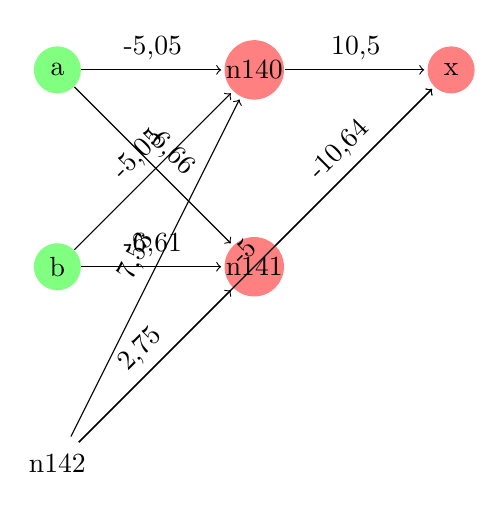
\begin{tikzpicture}[shorten >=1pt,->,draw=black!,node distance=2.5cm]
\tikzstyle{neuron}=[circle,fill=black!25,minimum size=17pt,inner sep=0pt]
\tikzstyle{constant}=[neuron, fill=white!50];
\tikzstyle{sigmoid}=[neuron, fill=red!50];
\tikzstyle{identity}=[neuron, fill=green!50];
\node [identity] (a) {a};
\node [identity,below of=a] (b) {b};
\node [constant,below of=b] (n142) {n142};
\node [sigmoid,right of=a] (n140) {n140};
\node [sigmoid,below of=n140] (n141) {n141};
\node [sigmoid,right of=n140] (x) {x};
\path[every node/.style={sloped,anchor=south,auto=false}]
(n142) edge node {-5} (x)
(n142) edge node {7,53} (n140)
(n142) edge node {2,75} (n141)
(n140) edge node {10,5} (x)
(n141) edge node {-10,64} (x)
(a) edge node {-6,66} (n141)
(a) edge node {-5,05} (n140)
(b) edge node {-5,05} (n140)
(b) edge node {-6,61} (n141)
;\end{tikzpicture}
\end{document}